\documentclass[modern]{aastex61}

%\pdfoutput=1 %for arXiv submission
\usepackage{amsmath,amstext}
\usepackage{graphicx}
%\usepackage[T1]{fontenc}
%\usepackage{apjfonts} 
\usepackage[figure,figure*]{hypcap}
%\usepackage{courier}
\PassOptionsToPackage{hyphens}{url}
\usepackage{hyperref}
%\usepackage[marginpar=2cm]{geometry}
%\usepackage[colorinlistoftodos]{todonotes}
\renewcommand*{\sectionautorefname}{Section} %for \autoref
\renewcommand*{\subsectionautorefname}{Section} %for \autoref
\expandafter\def\expandafter\UrlBreaks\expandafter{\UrlBreaks% save the current one
  \do\a\do\b\do\c\do\d\do\e\do\f\do\g\do\h\do\i\do\j%
  \do\k\do\l\do\m\do\n\do\o\do\p\do\q\do\r\do\s\do\t%
  \do\u\do\v\do\w\do\x\do\y\do\z\do\A\do\B\do\C\do\D%
  \do\E\do\F\do\G\do\H\do\I\do\J\do\K\do\L\do\M\do\N%
  \do\O\do\P\do\Q\do\R\do\S\do\T\do\U\do\V\do\W\do\X%
  \do\Y\do\Z\do\*\do\-\do\~\do\'\do\"\do\-}%


%\let\above\relax

\begin{document}

\title{Testing the LSST DM Stack on Deep Lens Survey Data}

\author{Imran Hasan, Perry Gee, Tony Tyson}
\collaboration{Physics Department, University of California,
One Shields Ave., Davis, CA 95616} 
\date{September 2017}


\email{ishasan@ucdavis.edu, pgee2000@gmail.com, tyson@physics.ucdavis.edu}


\begin{abstract}
We use version 13.0.9 of the LSST DM stack to reduce optical $R$ band data taken with the KPNO 4-meter telescope for the Deep Lens Survey (DLS). Because this data set achieves an LSST like depth and has been studied and characterized exhaustively over the past decade, it provides an ideal setting to evaluate the performance of the LSST DM stack. In this report we examine registration, WCS fitting, and image co-addition of DLS data with the LSST DM stack. Aside from using a customized Instrument Signature Removal package, we are successful in using the DM stack to process imaging data of a 40 x 40 square arcminute subset of the DLS data, ultimately creating a coadd image. We find the astrometric solutions on individual chips have typical errors $<$15 miliarcseconds, demonstrating the effectiveness of the {\tt\string Jointcal} package. Indeed, our findings in this regard on the DLS data are consistent with similar investigations on HSC and CFHT data.  

A closer look at the astrometry data set shows it contains larger errors in Right Ascension than Declination. Further examination indicates these errors are likely due to a guider problem with the telescope, and not the result of proper motions of stars, or a problem with the DM stack itself.

Finally, we produce a coadd using the reduced data. Our coadd is approximately 40 square arcminutes-much larger than the coadds typically created with the stack. Creating a large image stretched our machines to their limits, and we believe a dearth of system resources lead to coadd creation Task not finishing. In spite of this, the coadd produced by the stack is of comparable quality to its counterpart produced by the DLS team in previous analysis in terms of depth, and ability to remove artifacts which do not correspond to true astrophysical objects. However issues were encountered with {\tt\string SafeClip}.    
\end{abstract}

\section{Introduction}
The reprocessing effort using the LSST DM stack being undertaken by the community is key in validating the data management software being developed for the LSST. Surveys like SDSS, DES, and CFHT are being re-reduced and examined to ensure previous results are reproduced.  Because systematics are often specific to the details of the data acquisition, it will be important to test the DM stack using data representative of the LSST survey.  To aid in this endeavor, we have undertaken the task of reprocessing the Deep Lens Survey (DLS) with the LSST data management pipeline. The DLS is representative of the data that LSST will obtain, since it is deep
%\todo[size=\tiny]{xxx Should this be R?}%
(complete to 26th $R$ magnitude, covering a wide redshift range for galaxies), and the data were taken in the same way planned for LSST, using quasi-random shift-and-stare imaging and where one band was given priority in good seeing and for photometric and image quality uniformity.  In \S 2 we briefly discuss the telescope, camera, and data taken for the survey. In \S 3 we detail the steps taken to reduce the data. \S 4 details the performance of DM astrometric fitting. Finally, in \S 5 different methods of image co-addition are weighed. 
%Introduction text. \cite{1931ApJ....74...43H}.

\section{The DLS}
The DLS is a 20 square degree optical survey\footnote{dls.physics.ucdavis.edu/} consisting of five different 2 x 2 degree fields. Each field is subdivided into nine camera fields of view: 40 x 40 square arcminute subfields. Observations were made using the Mosaic 1.0 camera on the KPNO 4-meter and the Mosaic 2 camera on the CTIO 4-meter, with optical $B, V, R,$ and $z$ bands. In this work, we deal exclusively with R band data taken with the KPNO 4-m + Mosaic 1.0 and corresponding to field F2 (centered on RA: 09:18:00, DEC: +30:00:00 in equatorial coordinates and l = 197, b = 44 in galactic coordinates), subfield p23. See the DLS webpage or \cite{2012MNRAS.421.2251W} for a discussion of the photometric calibration and further specifics of the survey. 

The Mosaic 1.0 camera consists of a 4 x 2 grid of 2k x 4k CCDs. The plate scale of the CCDs is $\sim$ 0.26 arcseconds/pixel at the center of the field of view (FOV). $R$ band observations were made exclusively in sub-arcsecond seeing conditions. In total 21 pointings are made to this subfield between the years 2000 and 2003. In addition, pointings from neighboring subfields are also included where positional dithering caused them to overlap F2p23. In our approach we have created a description of the Mosaic 1 camera, obs mosaic, in the LSST framework and style of other cameras, along with a mapper class which allows a data butler to fetch information for this camera. 

\section{CCD processing}
The high level command line task
%\todo[size=\tiny]{How about if we use the actual task names in the code to refer to tasks, including leading caps?}%
{\tt\string ProcessCcd} is typically used to operate on raw data taken from an exposure and ultimately produce a data product suitable for scientific measurement. This task operates on individual exposures taken on each of the 8 detectors. {\tt\string ProcessCcd} consists of three other subtasks: {\tt\string ISR} (instrument signature removal), {\tt\string CharacterizeImage}, and {\tt\string Calibrate}. A camera specific {\tt\string ISR} task was written and used in lieu of the {\tt\string IsrTask} which is called by {\tt\string ProcessCcd} by default. The remaining tasks and subtasks therein remain unaltered and are used to reduce the individual exposures chip-by-chip \cite{2017arXiv170506766B}.

Bias correction, de-fringing, pupil correction, and flat-fielding are done during the original DLS pre-processing. Our custom ISR task makes use of this previous work, fetching these images using the "preprocessed" dataset defined specifically for the obs\_mosaic camera.

The {\tt\string MosaicPreprocessedIsrTask} performs the following functions:

%\todo[size=\tiny]{Imran, is there a way to make this into a bulleted list?}%
\begin{itemize}
\item Create a masked image for each CCD for a given field, subfield, date, and object.
\item Marks as SAT pixels to be treated as saturated.
\item Makes as BAD pixels so marked in bpm file for the observatory and year.
\item Marks as SUSPECT pixels which are contained in the DLS manual exclusion regions.
\item Does fixups of the GAIN, RDNOISE, and BORESIGHTRADEC for observations which lack them.
\item Calls updateVariance to create a variance plane for each image.
\end{itemize}
\subsection{How saturated pixels were marked}
Pixels were marked as saturated when they exceeded 85\% of the values typically found in the bloom regions around bright stars. Unfortunately, this value is not always consistent across a CCD or between different exposures with the same detector. And in some images blooms appeared at levels lower than the centers of what appeared to be unsaturated stars. Marking such stars as saturated in turn caused problems with the astrometric fitting.
We were able to solve this problem by setting the SAT higher in some cases. Unfortunately, doing this leaves blooms from some bright stars unmasked. We decided that this would be acceptable, as the DLS data includes a set of automatically generated bright object masks which can later be used to mask out these areas.

\subsection{Automatically generated bright object masks}
These masks were generated by the original DLS pipeline to mask areas when more than half of the exposures of a given area were infected by blooms from bright stars. The blooms are easily identified by their shapes, which begin at the centers of bright stars and extend along the readout columns in both directions.

\subsection{Manual exclusion masks}
The DLS data also includes a set of manually produced masks for excluding artifacts which appear in individual visits, such as satellite trails, reflections of bright objects from the edges of CCDs, or patterns of bright or dark pixels created by one-time problems with the detector electronics. The manual exclusion regions were created by manually examining all of the raw images and marking problem areas.
We mark these regions as SUSPECT in our {\tt\string calexps} so that we can chose later to exclude them from the coadds.

\subsection{Calibration of individual images}
One of the data products produced by ProcessCcd is a {\tt\string calexp}: a version of the raw image that has been run through instrument signature removal, is background subtracted, and includes objects such as a PSF model and a WCS. The {\tt\string calexp} WCS is created by refining the WCS initially provided by the telescope when the raw data were collected. In the refining process, detected sources are calibrated against a reference star catalog, in this case the sdss-dr9-fink-v5b catalog. A detection catalog, with equatorial coordinates provided by the Calibration process, is also provided by {\tt\string ProcessCcd} in the {\tt\string src} dataset, which by default uses the {\tt\string meas\_astrom} package. The astrometric correction can be refined further still by using the {\tt\string Jointcal} package. {\tt\string Jointcal} produces an additional WCS dataset, which may replace the original WCS during coaddition. In the following section, we evaluate the performance of the {\tt\string Calibration} task and any improvements provided by {\tt\string Jointcal}.

%\todo[size=\tiny]{xxx Not sure what "detrended" means}%
\section{meas\_astrom and jointcal performance}
Obtaining precise source registration on individual {\tt\string calexps} is crucial. Errors and inconsistencies in the astrometry on individual {\tt\string calexps} can systematically infect shape measurements on any coadd they are used to construct. Below we discuss our examination of two astrometric fitting packages used in the stack, {\tt\string meas\_astrom} and {\tt\string Jointcal}. 

First we match unblended objects with extendedness values of 0 from each of the individual {\tt\string src} catalogs against the SDSS DR9 Fink Catalog. We utilize the DM stack's {\tt\string matchRaDec} function with a tolerance of 0.5 arcseconds, recording only the closest matches to do so. The resulting sources in the matched catalog are considered to be stars. 

Second, we identify repeated observations of individual stars. All {\tt\string src} stars which matched against the same SDSS star in the DR9 Fink catalog are considered to be repeated observations of the same {\tt\string src} star at different epochs. After this step, the SDSS DR9 Fink Catalog is no longer used. 

Third, we assess how mutually consistent the astrometry for stars is over different epochs, using the following procedure. We only consider stars which have been observed in at least 8 epochs. The first instance of this star's astrometry in the match catalog from the first step is arbitrarily chosen to serve as a reference. The angular distance between the reference epoch and all other epochs is calculated, and the median of these distances is ultimately saved. The distribution of all such medians is obtained by repeating this for all stars, thus examining the consistency of the astrometric fit using the {\tt\string meas\_astrom} algorithm.

A second test is then performed, repeating the above procedure with one amendment. In the first step, the {\tt\string src} detection catalogs have their registrations refined by using the {\tt\string Jointcal} WCS, using {\tt\string afwTable.updateWcs}. The rest of the first, second, and third steps are carried out exactly as discussed above. This creates a distribution of median separations, this time probing the consistency of astrometric fitting using {\tt\string Jointcal}.

In Figure 1, the distribution of the median astrometric error is shown for both algorithms. {\tt\string Jointcal} clearly improves upon the {\tt\string meas\_astrom} algorithm. In the binning used in Figure 1 the peak of the {\tt\string meas\_astom} distribution is 22.5 milliarcseconds while the peak in the {\tt\string Jointcal} distribution is 13 milliarcseconds -- significantly smaller. These plots indicate the relative astrometry is highly consistent from exposure to exposure for a particular star. Lastly, these improvements are consistent with results from a similar study using CFHT data
%\todo[size=\tiny]{xxx These urls don't fit in the text}%
(\url{https://community.lsst.org/t/some-numbers-and-plots-on-the-astrometry/1592}) and HSC data (\url{https://community.lsst.org/t/some-results-on-jointcal-running-on-hsc-data/2132}).

\begin{figure}
   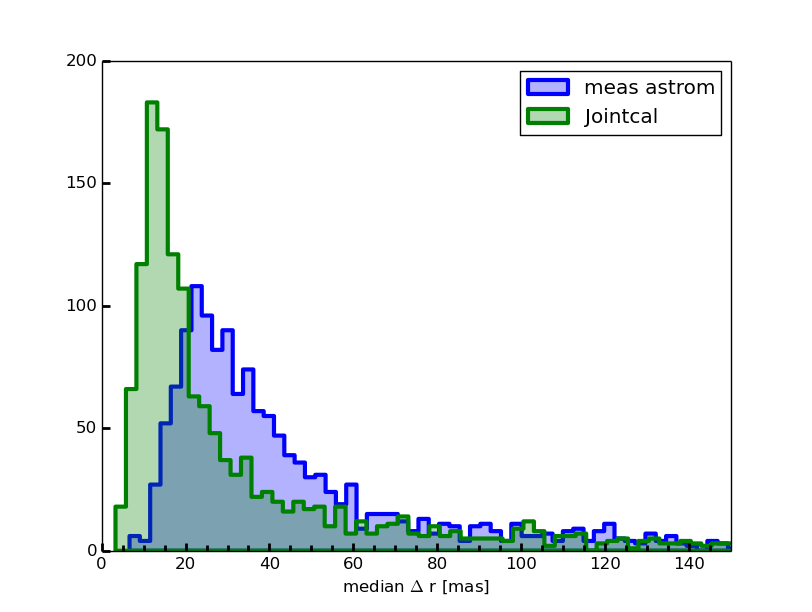
\includegraphics[width=.9\textwidth]{jc_vs_measastrom.png}
	\caption{We assess the consistency of the astrometry on {\tt\string calexps} with and without {\tt\string Jointcal}. The distribution of the median difference between a reference observation of a star and its subsequent observations at different epochs is shown. Using {\tt\string Jointcal} improves upon {\tt\string meas\_astrom}, and makes the registration of sources over time more consistent.}
\end{figure}

Analysis of DC1 data showed astrometric errors due to proper motions. We now investigate for the presence of a similar signal in the DLS data. The same match catalog constructed to produce the green {\tt\string Jointcal} curve in Figure 1 is used again. In this examination, however, we do not record the median change in position for a star with respect to an arbitrarily selected reference observation. Instead, the earliest epoch observation of a star is chosen as its reference position. The angular distance between the earliest epoch observation and all subsequent observations are calculated. In particular, we record the changes in RA and Dec separately. 

\begin{figure}[h!]
    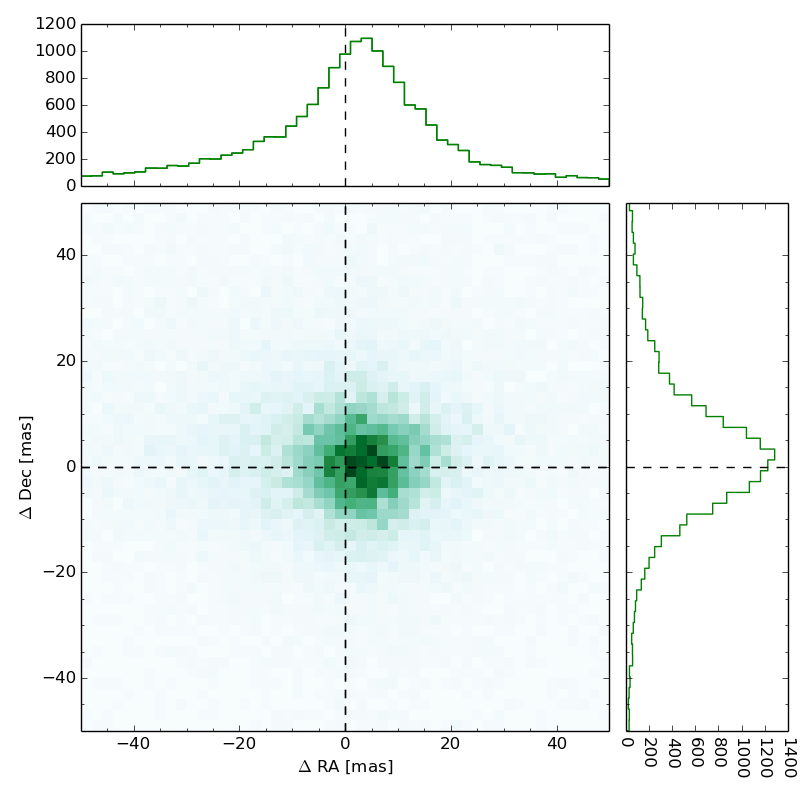
\includegraphics[width=.9\textwidth]{astrom_ra_dec_internal.png}
    \caption{2d histogram of the change in RA and Dec, along with 1d histograms of the marginalized distributions. The reference coordinates used are the earliest epoch detection of the star in our catalog. The distributions of the change in both coordinates are shifted by $\sim$ 5 milliarcseconds.}
\end{figure}

In Figure 2 we show the joint distribution of changes in RA and Dec, along with the marginalized distributions for each coordinate individually. A systematic offset of a few milliarcseconds is observed in both coordinates, although the offset and width in the RA distribution is noticeably larger-particularly in the 2d histogram. An analysis of simulated data from DC1 has a similar trend with a bias of $\sim$ 20 milliarcseconds in both coordinates (\url{https://github.com/LSSTDESC/SSim_DC1/issues/43}), again with the RA data suffering more. 
We must highlight some of the differences between the analysis presented here and that of the DC1 data. We note that the DC1 astrometry plot was generated by comparing the measured positions of stars to the truth catalog used by catsim. Ultimately, the change in measured positions to the truth positions in DC1 data is attributed to the proper motions which were assigned to stars, by assuming a model. After all, stars move across the sky and changes in stellar positions over a 10 year observing campaign can be expected.  

We do not believe the offsets in our data can be attributed to proper motions, however. Switching between equatorial coordinates for galactic coordinates, the data from Figure 2 is replotted in Figure 3. In this coordinate space, we see an offset in the b direction. Given that the field imaged in this data contains stars primarily from the thick extended Milky Way disk and galactic halo, this seems to indicate a bulk motion of the observed stars out of the plane of the galaxy at a rate of $>$ 1 mas/yr. Such a scenario seems unlikely-if anything, one might expect to find a net azimuthal motion of stars in the disk. 

\begin{figure}[h!]
	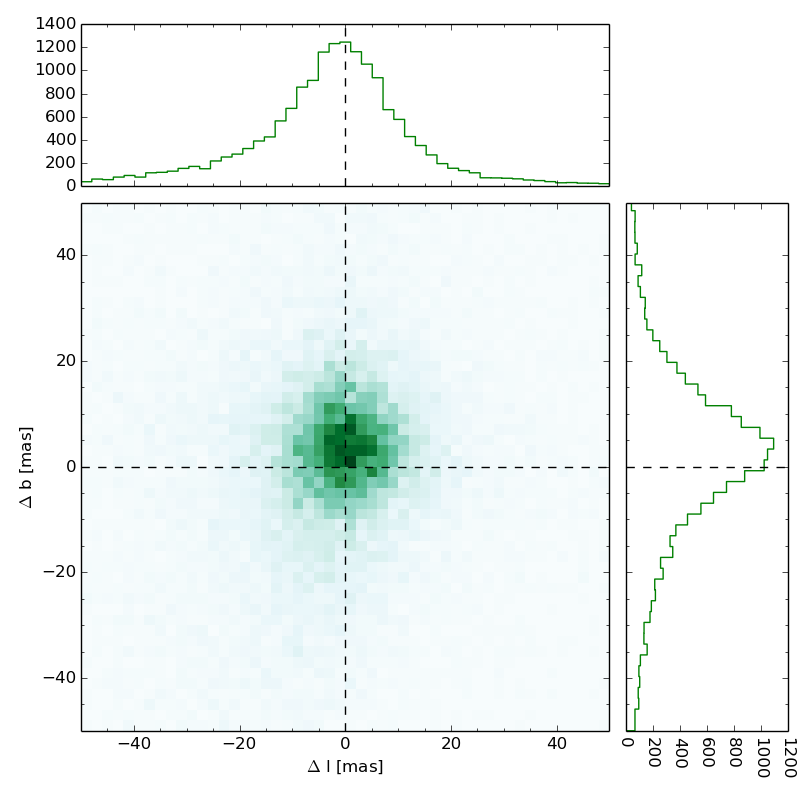
\includegraphics[width=.9\textwidth]{tech_memo_b_l.png}
    \caption{The same data used to create Figure 2 is transformed to galactic coordinates b, and l. In these coordinates, the b direction has an offset and wider dispersion, while the changes in the l position are largely symmetric and appear consistent with no offset. }
\end{figure}

An additional examination casts more doubt on the proper motion scenario for the DLS data set. Here we recreate Figure 2, using only data from 2000-11-27, 2000-12-19 and 2000-12-22, spanning over approximately one month. The systematic offsets on the order of a few miliarcseconds persist. We argue that the continued presence of the offsets in the distributions, in spite of significantly reducing the time span considered, arise from comparing astrometric errors relative to the first exposure which served as a reference, and not from proper motions. 

\begin{figure}[ht!]
    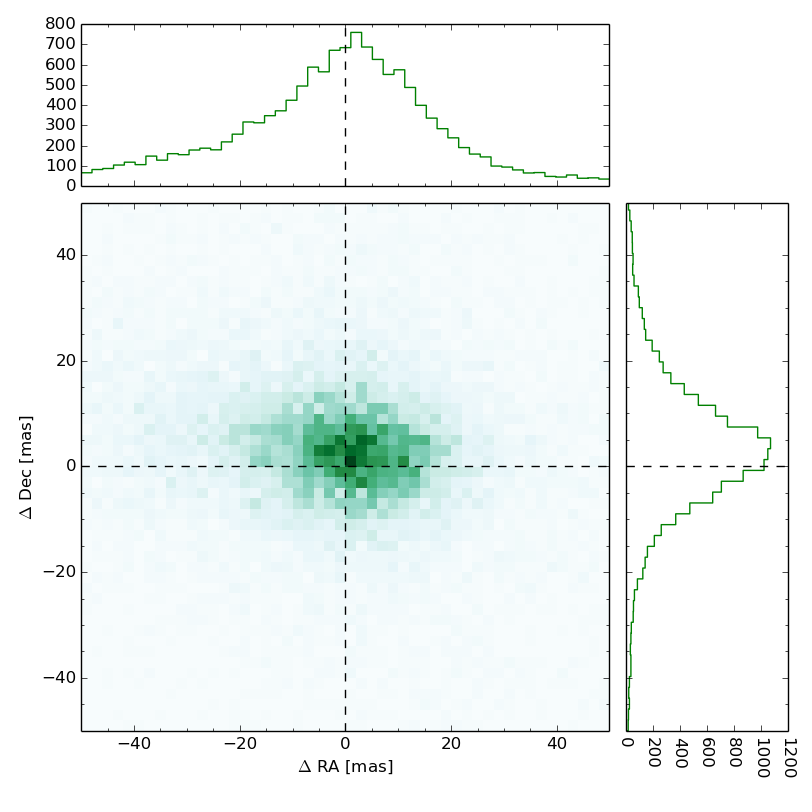
\includegraphics[width=.9\textwidth]{ra_dec_20001127_20001219_20001222.png}
    \caption{We recreate Figure 1, this time restricting our sample to observations made on 2000-11-27, 2000-12-19, and 2000-12-22. Systematic offsets in the distribution persist, although the offset in Dec is now larger than that in RA. Because these observations happened over the course of a month, it is unrealistic for proper motions to give rise to 5 miliarcsecond changes in position.}
\end{figure}

We now assess {\tt\string Jointcal} astrometry coordinate by coordinate, disregarding time dependence. We repeat the procedure used to create Figure 2 with the following difference: instead of choosing the earliest epoch observation of a star to serve as a reference, we randomly select the epoch which is used as a reference for each star. This places all epochs on equal footing, instead of choosing one as a reference against which all are compared. The resulting 2d and 1d histograms are shown in Figure 5. The distributions show no indication of bias or systematic offset, but do show larger dispersion in RA than Dec. 

\begin{figure}
	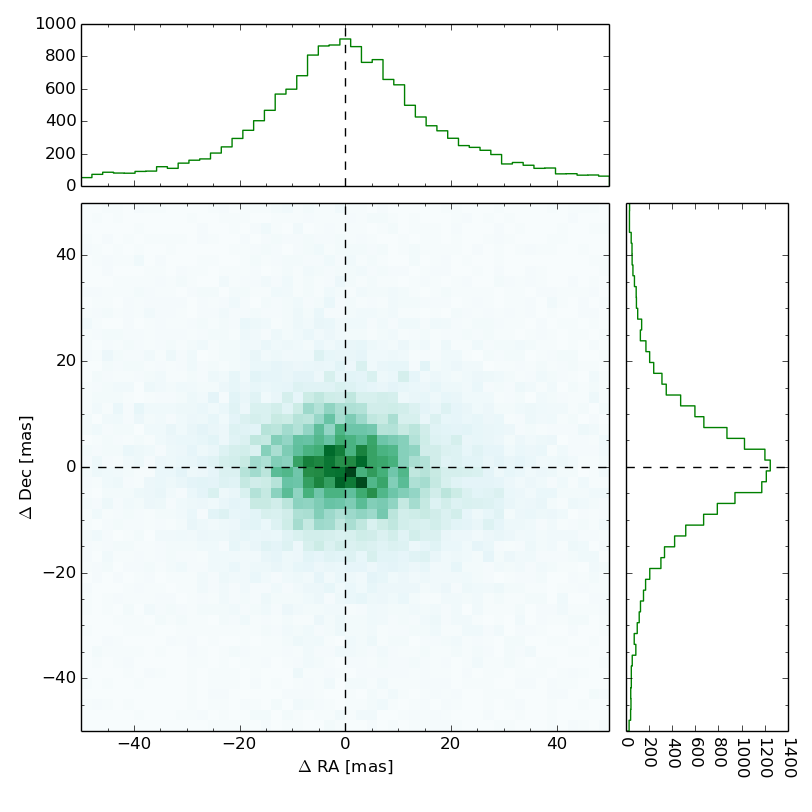
\includegraphics[width=.9\textwidth]{ra_dec_random.png}
    \caption{2d histogram of changes in the astrometry of stars, along with marginalized 1d histograms for each coordinate. This Figure differs from Figure 2 in that the reference epochs are chosen at random here, instead of using the earliest epoch. Randomizing the reference epoch 'washes out' any time-varying errors associated with the data. The resulting distributions are largely symmetric and have peaks consistent with 0 offset, and continue to have a larger dispersion in RA.}
\end{figure}

We now consider the wider dispersion in the RA direction exhibited in Figures 2, 4 and 5. Errors with the guide system may have played a role in this feature; the typical exposure time is 900 seconds and guide errors which are systematically worse in the RA direction during integration can lead to smearing. Under such a scenario, the widths of stars are expected to be systematically larger in the RA direction. 
This is indeed the case. The Mosaic 1 camera is an equatorial telescope, with the y direction on the its CCDs running parallel with RA and the x direction running parallel with Dec. In Figure 4, the second moments in the x and y direction are measured with the SDSS shape measurement plug-in, and are noticeably larger in the y/RA direction than the x/Dec direction. 
Comments in the observing logs from the DLS observing champaign are telling as well. Problems with guiding and telescope pointing for the Mayall 4-m were noted during the time this data were collected. Taking all of this information together, we draw the following conclusion: while we observe a similar offset in the $\Delta$RA/$\Delta$Dec distributions to the DC1 data, the DLS offsets do not originate from proper motions of stars. Instead, they can be attributed to imperfect guiding during integration. Additionally, we remark that in private correspondence with Dominique Boutigny, we are shown that HSC data shows no bias in its residuals in RA or Dec. Finally, Dave Monet's analysis of DECam data using {\tt\string Jointcal} shows no bias in Ra or Dec residuals either.
In all, we believe our work ultimately indicates {\tt\string Jointcal} is consistent and accurate, improves upon {\tt\string meas\_astrom}, and gives better astrometry than that achieved in previous DLS analysis. 

\begin{figure}
    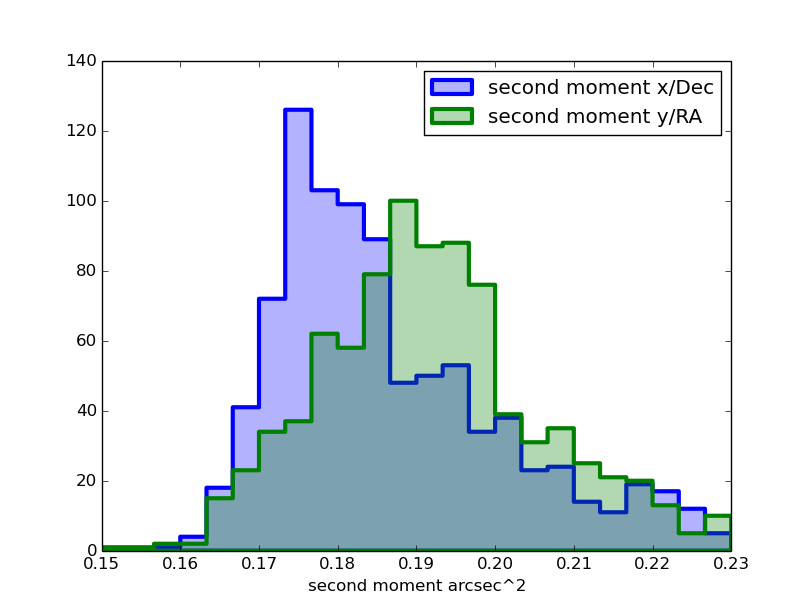
\includegraphics[width=.9\textwidth]{second_moments.png}
    \caption{Distributions for the median second moments of stars in this work in the x and y directions as measured by the SDSS Shape plug-in. The y direction of our CCDs run parallel with RA, and x direction run parallel with Dec. We note that stars are noticeably larger in the Y/RA direction than the X/Dec direction. This systematic difference in size may explained by tracking error in the telescope during integration. The KPNO 4-m telescope used to collect data in this work is an equatorial mount telescope, changing Hour Angle (HA) as 900 second exposures are taken. Jitter or oscillations in tracking may give rise to a smearing of stars, ultimately making them wider in the Y/RA direction.}
\end{figure}

\section{coaddition of exposures}
The {\tt\string Jointcal} astrometry was used to create a coadd of the DLS subfield F2 p23 using a 3 sigma clip mean. The 3 sigma clip mean is of most interest to us, since previous analysis of the DLS data used this technique as well. However, a cursory investigation of {\tt\string SafeClip} coadd technique was performed and is discussed further below. 
The 3 sigma clip coadd is largely successful in removing artifacts, ghosts, and satellite trails. A by-eye side by side comparison between the coadd of F2 p23 produced by the DM stack and that produced in previous DLS analysis shows they are of comparable quality in this regard.
Note, however, that the DLS pipeline also used both the automatically generated bright object masks and the manually generated one-time artifact masks to improve the quality of the coadds. The exclusion of objects in the vicinity of bright object blooms improved the quality of the DLS catalogs. Except in a few cases, the 3-sigma clip appeared to remove most one-time artifacts successfully.

%\bigskip
%\subsection{coadd astrometry}
%In previous sections the consistency of source registration was examined in a chip-by-chip basis. To see if the fidelity of the astrometry propagates through to coaddition, we compare detections on the coaddd to those in {\tt\string src} catalogs. The algorithm is as follows. The command line task {\tt\string MeasureCoaddSources} is run. The coadd detection catalog is matched against the SDSS-Dr9 Fink catalog to identify stellar sources. The stellar sources in the coadd catalog are used to construct a reference catalog. The reference catalog is then matched against all the {\tt\string src} catalogs (whose registrations are updated with {\tt\string Jointcal} WCS). Matches are then grouped by their unique identifier in the reference catalog. The RMS of the distances between all {\tt\string src} stars and their matched star in the coadd is also calculated.  

%Additionally, the mean RA and Dec positions of stars is constructed from all {\tt\string src} stars which were identified as single epoch observations of the same star from the reference catalog is calculated to yield an average position. The scatter from the . The resulting distributions rms in separation with respect to the coadd catalog are displayed in Figure 7.

%\begin{figure}
%    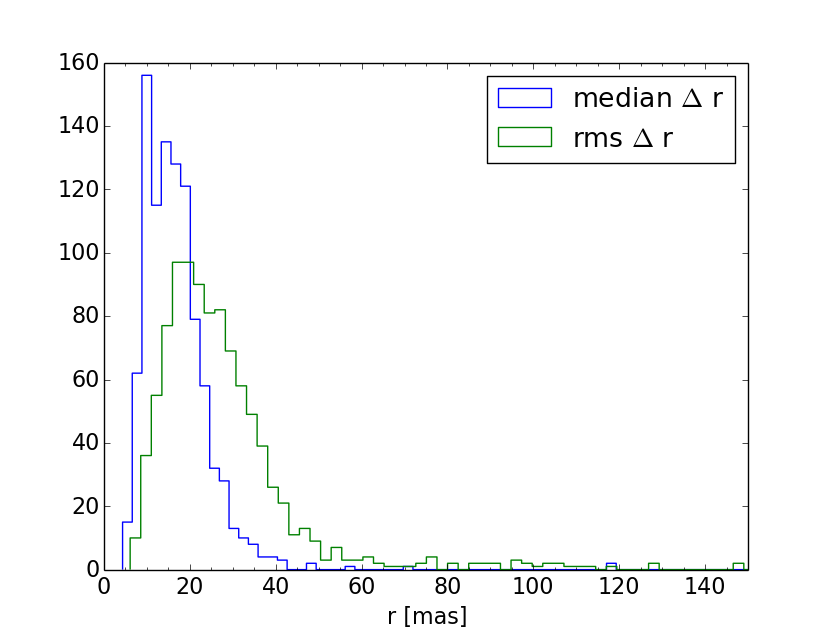
\includegraphics[width=.95\textwidth]{coadd_astrom_median_rms.png}
%   	\caption{The distributions of the median separation of {\tt\string src} catalog stars to their coadd detection, and the rms of the separations is shown. The means of the median and rms distributions are 16.99 mas and 29.9 mas respectively. The distributions indicate the fidelity of the astrometric fitting has propagated through to the coadd's registration.}
%\end{figure}

%Scatter is also considered for right ascension and declination separately. In addition to recording the median angular distance from {\tt\string src} stars to their matched coadd stars, the median difference in right ascension and declination is also recorded. The distributions are noticeably different; the RA scatter is asymmetric and broader than the Dec scatter. 

\newpage
\bigskip
\bigskip
%perry's discussion of safeClipCoadd can go in this 
\section{co-addition techniques: a comparison of different algorithms}
Co-addition in the stack utilizes an object called skymap, which subdivides a region of the sky in large regions referred to as tracts, which are then subdivided into patches. The sizes of tracts and patches, and number of patches in an individual patch can be defined by the user. To test co-addition, we produced a co-add for DLS field F2 using a skymap defined in the following way. Our skymap contains a tract the same approximate size of, and centered on, the DLS field F2. The patches belonging to this tract are also of similar size and position to the DLS subfields of F2. These patches are 10000x10000 pixel images with a scale of approximately 0.257 arcsecs per pixel. This produces a coadd image the size of the 40 arcsec square DLS subfield plus a small amount of inter-subfield overlap. The number of component exposures which are incorporated into each image varies from patch to patch, from 213-334, depending on the patch. There were 249 individual {\tt\string calexps} included in patch 2,1, the equivalent of DLS subfield F2p23.

We experienced significant difficulties at this patch size with {\tt\string AssembleCoadd}, particularly with the {\tt\string SafeClip} algorithm. (See the Appendix for more details). We ultimately divided the patches into regions which were approximately 2500x2500 pixels, or a quarter of a subfield.
\subsection{System limitations with the {\tt\string AssembleCoadd} Task}
Our first attempts to run a complete {\tt\string AssembleCoadd} were with stack version 12.3.1, using the default configuration for {\tt\string AssembleCoadd}: this configuration utilizes the {\tt\string SafeClip} algorithm to exclude outlier pixels. The {\tt\string AssembleCoadd} task ran for quite some time, eventually going into "D" status in top. We once saw the algorithm complete after running for over a day, but in general, the algorithm does not appear to complete successfully on our machines.

We have not investigated this thoroughly, but we believe that the problems have to do with inadequate system resources, perhaps memory or swap. The system has 32GB of memory and 32GB of preallocated swap.  It is also possible that the computer is thrashing, as there appears to be a huge amounts of I/O at times during the Task execution.

We repeated our tests more carefully using version 13.0.9 of pipe\_tasks, and recorded the "top" information for this writeup. See the appendix for a detailed account.

\bigskip
\subsection{Successful configurations}
To cure our problem with coadd failures, we tried instead to run {\tt\string AssembleCoadd} with the {\tt\string LegacyCoadd} option, which employs a simpler 3-sigma clip. This outlier rejection also appears to stretch our system to its limits, but the 3-sigma clip does always seem to complete as long as there are no other large consumers of system resources running at the same time.
We were also successful running both clipping techniques with the smaller quarter subfield patch size.  
\subsection{Some examples of LegacyCoadd vs. SafeClipCoadd}
The original DLS pipeline used a 3-sigma clipping algorithm, but one which was modified to not remove the centers of stars, where the core often appears as an outlier. Though we are interested in using the Legacy clipping algorithm for comparison, it is also important for us to evaluate the {\tt\string SafeClip} algorithm being used for HSC processing.
With the DLS data, which has up to 22 measurements of each coadd pixel, we found many cases where the {\tt\string SafeClip} algorithm failed to remove obvious artifacts. We are unsure whether changing the statistical config parameters might improve the performance of {\tt\string SafeClip}.

Shown below are examples were we think that {\tt\string LegacyCoadd} succeeded in eliminating exposure artifacts, while {\tt\string SafeClip} did not. We have not investigated the reasons for these problems, but include these examples hoping that they will be useful to the collaboration.  Note that the direction of readout is horizontal.  The {\tt\string LegacyCoadd} result is shown on the left, while the {\tt\string SafeClip} result is on the right.

Figure 7 (a) shows a problem resulting from a dark row which was 1 row wide and about 40 columns long on a single {\tt\string calexp}.  This was 1 or 21 {\tt\string calexps} used to build this part of the coadd. It was not marked as bad in the telescope bad pixel map. These pixels are unmarked in the {\tt\string calexp} mask, but some of the pixels immediately to the right are marked as CR and INTRP, so the curious artifact in the coadd is probably the result of CR repair of the image during {\tt\string ISR}.  The 3-sigma clip removed this artifact.

\begin{figure*}
\gridline{\fig{fig1.png}{0.5\textwidth}{(a)}
          \fig{fig2.png}{0.5\textwidth}{(b)}
		}
\gridline{
		\fig{fig3.png}{0.5\textwidth}{(c)}
        \fig{fig5.png}{0.5\textwidth}{(d)}
	}
\caption{We compare and contrast the performance of {\tt\string LegacyCoadd} and {\tt\string SafeClip} on removing artifacts, including satellite trails and blooms.}
\end{figure*}

Figure 7 (b) shows line artifacts which frequently appear on the boundary between saturated areas and unsaturated areas, in particular at the borders of the bloom areas of very bright stars. The {\tt\string LegacyCoadd} does a better job of removing them than does the {\tt\string SafeClip}.

Figure 7 (c) shows an artifact which resulted from a bright 4 or 5 pixel wide band in the exposure which crossed two CCDs. It appears on only 1 of 19 exposures used to build this coadd. The bright band is perpendicular to the readout direction, and is only about 1/3 of the saturation level.

Figure 7 (d) shows an area where satellite trails appear in the {\tt\string calexps} which make up this coadd. Only one is not correctly clipped. They all have the same mask values surrounding the lengths of the trails.  They do vary in intensity, but none are close to saturation. The one which did not get masked is neither the brightest nor the faintest.

\bigskip

\section{Summary}
In summary, we reprocess a subset of the DLS data using the LSST DM stack, ultimately creating a coadd and coadd measurement catalog. Examination of detection catalogs provided by the stack demonstrate an astronomic precision which exceeds former results obtained in previous analysis of the DLS. We show that implementing the simultaneous astrometry package {\tt\string Jointcal} is key in achieving this precision. 

We find an anomaly in the astrometric error distribution, with larger error in the RA direction. This is independent of astrometric reference frame.  It is unlikely to be caused by proper motion stars, and more likely results from imperfect guiding.

Some technical hurdles are encountered in creating the coadd while using the Legacy option, possibly due to a lack of resources on the machines used for this work (a more in depth discussion can be found in the appendix), though they are overcome. A cursory investigation of the {\tt\string SafeClip} coaddition method reveals some failures to remove artifacts and additional technical problems. We note a fine tuning of the {\tt\string SafeClip} algorithm to DLS specific needs may ameliorate some of the problems encountered; however we do not investigate this further. 

\bigskip


\bibliographystyle{yahapj}
\bibliography{references}

\appendix
\section{Discussion of system capacity problems with AssembleCoadd}
This is a record of some of the problems we encountered running the {\tt\string AssembleCoadd} task, both with 3-sigma clipping and {\tt\string SafeClip}. The top logs were created while we were looking for a solution to the problems we encountered with various task configuration.
\subsection{Assemble Coadd with default config}
We did most of our original work with a version 12.3.1 stack.  However, we came back later to check our results with 13.0.9, and took some top logs to confirm that we were still having the same problems.  Running patch 2,1 coadd (DLS subfield F2p23) with {\tt\string SafeClipCoadd}, we reached the following state after many hours of execution.  Note the the actual elapsed time was at least 36 hours -- the TIME+ entry is cpu time, not elapsed time.

\begin{small}
\begin{verbatim}
Tasks: 364 total,   1 running, 363 sleeping,   0 stopped,   0 zombie
Cpu(s):  0.0 us,  0.1 sy,  0.0 ni, 91.6 id,  8.2 wa,  0.0 hi,  0.0 si,  0.0 st
KiB Mem:  32948336 total, 32649588 used,   298748 free,     1724 buffers
KiB Swap: 78564832 total, 75636136 used,  2928696 free.  4271744 cached Mem
\end{verbatim}
\end{small}

Here is log of task resource use which was taken every 20 minutes. The task was allowed to run for about 36 hours before it was killed. The entries shown were collected during the first day.

\begin{small}
\begin{verbatim}
VIRT    RES    SHR    S  %CPU %MEM  TIME+      
1715992 260740 128148 R  99.0  0.8   0:11.20
3030484 1.163g 141052 R  69.4  3.7  15:38.38
10.976g 9.485g 141440 D  49.3 30.2  29:46.78
7477884 5.656g 141444 R  58.1 18.0  54:20.72
10.566g 9.090g 141444 R  48.2 28.9  66:23.97
8477888 6.609g 141444 D  26.3 21.0  90:53.53
13.425g 0.012t 141464 R  29.9 38.0 130:01.43
12.593g 0.011t 141464 R  44.6 35.4 143:27.40
9658300 7.726g 141464 R  78.2 24.6 156:44.98
6908292 5.112g 141464 R  46.6 16.3 169:58.13
4460640 2.778g 141464 R  36.3  8.8 183:12.37
60.299g 0.030t   5052 D  40.7 96.3 195:26.70
94.061g 0.029t   2116 D  50.8 95.2 202:55.51
94.061g 0.029t   2080 D  24.2 95.8 205:10.44
94.061g 0.029t   2080 D   3.6 95.4 206:54.34
94.061g 0.029t   2080 D  25.6 95.4 208:58.17
94.061g 0.029t   2076 R   5.9 94.1 214:56.81
94.061g 0.029t   2068 D  25.6 93.2 216:52.99
94.061g 0.028t   1936 D   5.0 91.9 220:21.73 
94.061g 0.027t   1916 D   4.3 87.4 224:58.89 
94.061g 0.029t   1932 D   6.0 94.3 227:50.19 
94.212g 0.027t   1808 R  93.3 86.8 232:04.02 
94.091g 0.029t   1936 D  12.1 93.6 234:08.56 
94.061g 0.028t   1944 D   4.6 92.3 236:59.73 
94.061g 0.029t   1944 D  12.2 93.4 239:06.16 
94.061g 0.028t   1940 D  24.8 92.0 243:12.36 
94.061g 0.029t   1940 R  34.3 93.5 245:31.43 
94.061g 0.029t   1940 D  11.6 93.5 247:10.51 
94.061g 0.029t   1944 D   4.0 93.4 250:14.82 
94.180g 0.029t   1824 R  65.0 92.9 255:36.13 
94.074g 0.028t   1944 R  41.9 92.1 257:25.35 
94.074g 0.028t   1944 D  18.5 92.5 259:03.34 
94.074g 0.027t   1940 D   6.1 86.9 262:25.31 
94.074g 0.028t   1940 D   6.0 91.9 264:43.29 
94.061g 0.029t   1944 R   6.1 93.7 284:05.20 
95.156g 0.029t    192 R  91.4 93.9 285:14.96 
95.156g 0.028t   2352 D   6.1 92.3 287:37.41 
\end{verbatim}
\end{small}

All entries after the last one shown were similar: a small CPU percentage, a very large VIRT and RES entry, and a state listed as "D".

\subsection{Assemble Coadd with LegacyCoadd option}
This configuration allowed us to run full subfield sized coadds, though they seemed to occasionally fail. At the time, other processes were running on the same machine, so we are not sure why they did not always succeed. The main thing is that we were able to get results from such trials, through they were also extremely slow and machine consumptive.

\subsection{Tests with a smaller subregionSize}
At Paul Price's suggestion, we tried reducing the {\tt\string subregionSize} to (1000,1000). This is 1/4 of the area used with the default config. While this configuration appeared to improve the VIRT and RES usage during most of the run, the Task still went into a "dead" state at the end of the assembly process. We believe this is during the final assemble process, since in successful runs (see below), the memory usage also rises sharply right at the end. In this unsuccessful run, the Task appeared to run for several hours without straining system resources, but in the end died with a top line which looked like this:

\begin{small}
\begin{verbatim}
safeClipAssembleCoadd INFO: Found 249 deepCoadd_directWarp
safeClipAssembleCoadd INFO: Assembling 249 deepCoadd_directWarp
safeClipAssembleCoadd INFO: Assembling 249 deepCoadd_directWarp
safeClipAssembleCoadd.clipDetection INFO: Detected 29035 positive sources to 2 sigma.
safeClipAssembleCoadd.clipDetection INFO: Detected 12824 negative sources to 2 sigma
safeClipAssembleCoadd INFO: Found 36771 potential clipped objects

3598980 1.830g  10024 D  30.3  5.8  55:35.80 python
4864612 3.036g  10024 D  35.7  9.7  65:22.23 python
4110312 2.312g   6824 D  47.4  7.4  75:23.42 python
4372420 2.562g   6824 R  31.8  8.2  85:15.61 python                                                       
3954452 2.164g   6824 R  47.3  6.9  95:04.38 python                                                       
5032580 3.186g   6540 D  72.6 10.1 104:48.31 python
6118520 4.214g   6176 R  34.9 13.4 114:37.27 python                                                       
4442732 2.609g   6176 D  31.7  8.3 124:41.01 python
4846536 2.982g   8072 R  29.8  9.5 135:34.59 python                                                       
6315292 4.383g   8040 D  47.6 13.9 145:57.37 python
6462556 4.526g   8040 R 100.0 14.4 156:29.39 python                                                       
4869972 3.005g   8040 R  32.1  9.6 167:16.99 python                                                       
6487168 4.546g   8040 D  36.0 14.5 177:41.85 python
7342636 5.365g   8040 R   0.0 17.1 188:14.23 python                                                       
5303568 3.417g   8040 R  30.0 10.9 198:49.12 python                                                       
6280136 4.352g   8040 R  30.9 13.8 209:20.97 python                                                       
5806308 3.900g   8040 R  35.6 12.4 220:00.18 python                                                       
7061384 5.097g   8040 R  49.2 16.2 230:22.42 python                                                       
7342636 5.365g   8040 R   0.0 17.1 240:58.76 python                                                       
6830916 4.858g   7416 R  24.6 15.5 251:08.39 python                                                        
26.906g 0.024t   8116 R 100.0 79.5 263:51.78 python                                                        
80.739g 0.029t   5080 D  12.1 96.0 274:22.41 python
94.062g 0.029t   2084 D   6.0 95.5 278:49.13 python                                                        
94.062g 0.029t   2084 D   0.0 95.1 280:30.75 python                                                        
94.062g 0.029t   2084 D   0.0 95.2 282:06.00 python                                                        
94.062g 0.029t   2084 D   5.8 95.2 283:55.72 python                                                        
94.062g 0.029t   2076 D   6.2 94.7 285:47.44 python                                                        
94.062g 0.029t   2076 D   4.8 94.7 287:55.85 python

\end{verbatim}
\end{small}

The last state shown, with the suddenly large VIRT and RES values, is the same as the "dead" state found when we first ran the algorithm.

\begin{small}
\begin{verbatim}
KiB Mem:  32948336 total, 32734896 used,   213440 free,      648 buffers
KiB Swap: 78564832 total, 66034528 used, 12530304 free.    22800 cached Mem

VIRT    RES       SHR S  %CPU %MEM TIME                                               
94.062g 0.029t   2084 D  23.8 94.7 281:34.20
\end{verbatim}
\end{small}

\subsection{successful runs using Legacy Coadd and a smaller patch size}
We discovered early in our trials that we could run {\tt\string SafeClipCoadd} and {\tt\string LegacyCoadd} much more quickly with a smaller patch size. We experimented with various patch sizes, and came to the conclusion that the largest patch we could get away with was about 1/4 of the size of a DLS subfield, or 2500x2500 pixels. This patch size allows us to successfully run both the {\tt\string SafeClip} and the 3-sigma clip algorithms. Using these smaller patches, we were able to do a comparison of the two algorithms on DLS data.

By comparison, the {\tt\string SafeClipCoadd} on the quarter sized patches does not use up all of memory or swap, and eventually completes assembly:
\begin{small}
\begin{verbatim}
VIRT    RES    SHR S  CPU MEM     TIME+ COMMAND

2650304 1.055g 143224 R  43.1  3.4   9:44.83 python                                       
2726592 0.997g  11604 D  70.4  3.2  13:15.98 python                                       
3179732 1.413g   8380 R  69.8  4.5  16:45.50 python                                       
3929764 2.097g   6340 R  72.8  6.7  20:23.87 python                                       
...
13.273g 0.011t   9140 R  77.3 36.9  24:15.75 python                                       
13.485g 0.012t   9208 R  99.7 37.6  29:15.12 python                                       
14.429g 0.012t  10712 R  76.7 40.5  33:05.16 python                                       
14.630g 0.013t   6504 R  63.2 40.9  36:14.77 python
\end{verbatim}
\end{small}
The elapsed time was approximately 50 minutes for this 2500x2500 image.

\end{document}